\documentclass[letterpaper,12pt]{article}
\usepackage{booktabs}
\usepackage{bm}
\usepackage{colortbl}
\usepackage{tabularx}
\usepackage{textcomp}
\usepackage{siunitx}
\usepackage{booktabs}
\usepackage{enumitem}
\usepackage{xcolor}
\usepackage{fancyhdr}
\usepackage{caption}
\usepackage{changepage}
\usepackage{amsmath} 
\usepackage{graphicx}
\usepackage{subcaption}
\usepackage[table]{xcolor} 
\usepackage[margin=1in,letterpaper]{geometry} % decreases margins
\usepackage{cite} % takes care of citations
\usepackage[final]{hyperref} % adds hyper links inside the generated pdf file
% Define the colors
\definecolor{linkcolor}{RGB}{0, 102, 204}
\definecolor{citecolor}{RGB}{34, 139, 34}
\definecolor{urlcolor}{RGB}{255, 69, 0}

% Setup hyperref
\hypersetup{
    colorlinks=false, % colored links
    linkcolor=linkcolor, % color for internal links
    citecolor=citecolor, % color for citations
    urlcolor=urlcolor, % color for URLs
    linkbordercolor=linkcolor, % color of box around links
}
\fancypagestyle{logoheader}{
    \fancyhf{}
    \fancyhead[L]{
\includegraphics[width = 3cm]{infn-art-science-universita-degli-studi-di-milano-bicocca-maintainer-universita-studi-milano-bicocca.png}}
    \renewcommand{\headrulewidth}{0pt}
    }
\usepackage{blindtext}
\graphicspath{{immagini/}}
%Required for inserting images
%++++++++++++++++++++++++++++++++++++++++
%Margini 



\begin{document}

\title{{\small Università degli studi Milano-Bicocca  Dipartimento di Fisica - Laboratorio II }\\
	Esperienza Circuiti II}
\author{F. Ballo, S. Franceschina, S. Dolci - Gruppo T1 39}
\date{\today}
\maketitle
\thispagestyle{logoheader}


\begin{abstract}
	Nella seguente relazione vengono presentati i risultati ottenuti dalla seconda esperienza del corso di Laboratorio II riguardante l'analisi di circuiti elettrici. L'obiettivo di questa esperienza era quello di studiare circuiti RC, RL e RLC in regimi di corrente impulsata (usando un onda quadra fornita da un generatore di funzioni). In particolare volendo verificare le leggi che descrivono questi circuiti, sono state effettuate misurazioni con oscilloscopio sull'andamento della differenza di potenziale ai capi dei vari componenti: resistenza, capacità e induttanza.

	\begin{adjustwidth}{-1cm}{-1cm}


	\end{adjustwidth}
\end{abstract}
\tableofcontents
\newpage

\section{Circuito RC}

\subsection{Configurazione del circuito e della strumentazione}
Di seguito abbiamo riportato lo schema \ref{fig:config_circuito} utilizzato per riprodurre il circuito RC in laboratorio con l'utilizzo di una bread-board e degli opportuni componenti, con l'obiettivo di verificare la seguente legge che descrive l'andamento della tensione in un circuito RC:
\begin{equation}
	\label{eq: Modello esponenziale}
	V(t) = V_0 \left(1  -e^{-\frac{t}{\tau}}\right)
\end{equation}
Per fare ciò abbiamo selezionato con un generatore di funzioni un segnale a onda quadra di frequenza $f$, per simulare l'apertura o chiusura del generatore, verificando che la durata dell'impulso sia abbastanza lunga da permettere alla capacità $C$ di caricarsi.
Per trovare la curva che descrive l'andamento di $V(t)$ è stato necessario campionare punto per punto il grafico che ci appare sull'oscilloscopio dopo aver  misurato con le sonde i segnali di tensione ai capi del resistore $R$ e capacità $C$. Prima delle misure abbiamo verificato la calibrazione di: oscilloscopio, generatore, sonde di misura e le "dimensioni" resistenza $R$ e capacità $C$.
\begin{figure}[h!]
	\centering
	\resizebox{0.5\textwidth}{!}{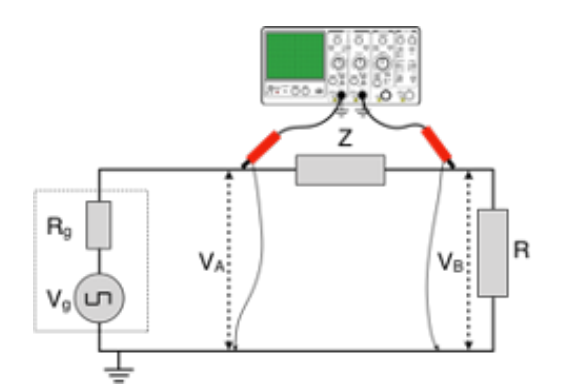
\includegraphics{configurazione_circuito.png}}
	\caption{Schema configurazione di circuito, Z rappresenta uno dei componenti tra R, C e L}
	\label{fig:config_circuito}
\end{figure}



Riuscire a verificare la legge prevista per il regime di circuito in questione permette di trovare la costante di tempo caratteristica \ref{costante tempo caratteristica}; conoscendo il valore di $R$ possiamo quindi stimare quanto vale la capacità $C$.
\begin{equation}
	\tau = RC
	\label{costante tempo caratteristica}
\end{equation}
\newpage



\subsection{Dati}
Di seguito riportiamo i dati e la configurazione del circuito RC studiato:
\begin{enumerate}[itemsep=1pt]
	\item Resistenza interna oscilloscopio $R_o = \SI{50}{\ohm}$
	\item Resistenza usata nel circuito $R = (67.1\pm0.1) \text{k}\Omega$
	\item Frequenza generatore $f = \SI{200}{\hertz}$
	\item Intervallo tensione $V_0= (1000.0 - 0000.0) \text{ mV}$
	\item Precisione oscilloscopio 0.004 V
\end{enumerate}


%Qui metterei i grafici di carica e scarica dei circuiti
\subsection{Analisi dati}
\begin{figure}[h]
	\centering
	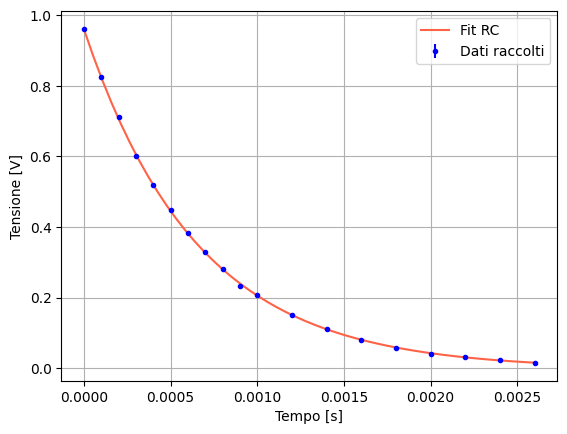
\includegraphics[width=0.8\textwidth]{RC.png} % Replace example-image with the filename of your image
	\caption{Grafico fit RC}
	\label{fig:fitRC}
\end{figure}
Per prima cosa abbiamo verificato la  misura  di C mediante un multimetro palmare, ottenendo: $$ C = (10 \pm 0.1)\ \text{nF}$$  valore che abbiamo usato per fare un confronto con quello ricavato dal fit.\\
Dopo aver raccolto i dati, abbiamo proceduto a interpolarli secondo la legge \eqref{eq: Modello esponenziale}, ottenendo i seguenti valori dei parametri:
\begin{align*}
	V_0  & = (963.7 \pm 3.1)\cdot 10^{-3}\ \text{V} \\
	\tau & = (652 \pm 6) \cdot 10^{-6}\ \text{s}
\end{align*}
Conoscendo la resistenza R, abbiamo calcolato $C = \frac{\tau}{R}$ e propagato le incertezze con l'opportuna formula:
$$ C_\text{calc}= (9.72 \pm 0.08) \cdot 10^{-9} \text{ F} \quad
	C_\text{attesa}= (10 \pm 0.1) \cdot 10^{-9} \text{F}
$$ \\


\subsection{Conclusioni circuito RC}
Il fit ritorna un valore del $\widetilde{\chi}^2 = 0.7$ e $p-value = 0.817$, il che indica una buona compatilità delle misure con il modello \eqref{eq: Modello esponenziale}\\

Eseguendo un test di compatibilità con la misura effettuata otteniamo $t = 1.02$. \\

La misura di C rientra entro poco più di una deviazione standard dalla misurazione effettuata, fornendo ulteriore conferma della bontà dell'adattamento.

\subsection{Discussione sulle incertezze}

La nostra stima delle incertezze è stata basata sulla precisione dell'oscilloscopio, che a seconda della scala di risoluzione variava da 2 a 20 mV. \\
In ciascun esperimento abbiamo tentato di selezionare il range dello strumento in modo che nello schermo fosse visibile tutta l'onda, senza mostrare regioni al di fuori del regime di interesse.\\
Per validare il nostro metodo, abbiamo eseguito una stima a posteriori delle incertezze, osservando che la variazione sull'incertezza era sempre compatibile con l'errore da noi utilizzato.
\newpage
\section{Circuito RL}

\subsection{Configurazione del circuito e della strumentazione}
L'obiettivo di questa sezione è applicare la stessa analisi seguita per il circuito $RC$ sostituendo la capacità con un induttanza $L$.
In questo circuito il modello che descrive l'andamento della tensione risulta essere:
\begin{equation}
	V(t) = V_0 \left(1  -e^{\frac{t}{\tau}}\right)
\end{equation}
Per le misurazioni abbiamo ripetuto lo stesso procedimento: selezionare con un generatore di funzioni un segnale a onda quadra di frequenza $f$, per simulare l'apertura o chiusura del generatore, verificando che la durata dell'impulso sia abbastanza lunga da permettere all'induttanza $L$ di caricarsi.
Per trovare la curva che descrive l'andamento di $V(t)$ abbiamo campionato punto per punto il grafico riportato dall'oscilloscopio dopo aver misurato con le sonde il segnale tensione, stavolta ai capi del resistore $R$ e induttanza $L$. Prima di effettuare le misure abbiamo verificato la calibrazione di: oscilloscopio, generatore, sonde di misura e "dimensioni" di resistenza $R$ e induttanza $L$ in rapporto alla resistenza interna dell'oscilloscopio.\\
Il nostro scopo è di nuovo quello di ricavare la costante di tempo caratteristica \ref{costante tempo caratt} per il regime di circuito in questione, conoscendo il valore di $R$ possiamo stimare quanto vale $L$.
\begin{equation}
	\tau = \frac{R}{L}
	\label{costante tempo caratt}
\end{equation}
\newpage

\subsection{Dati} %mancano le incertezze
Di seguito riportiamo i dati e la configurazione del circuito RL analizzato:
\begin{enumerate}[itemsep=1pt]
	\item Resistenza interna oscilloscopio $R_o = (50.0\pm0.1)\Omega$
	\item Resistenza circuito $R = (1000.01\pm0.01)\Omega$ %qual era la precisione della resistenza?
	\item Frequenza generatore $f = \SI{700}{\hertz}$
	\item Intervallo tensione $V_0= \pm (1000.0\pm0.1)\text{ mV}$
	\item Precisione oscilloscopio 	0.02


\end{enumerate}

\subsection{Analisi dati}

\begin{figure}[h]
	\centering
	\includegraphics[width=0.8\textwidth]{RL.png} % Replace example-image with the filename of your image
	\caption{Grafico fit RL}
	\label{fig:fitRL}
\end{figure}

Il processo di analisi è molto simile a quello effettuato in precedenza, tuttavia, non avendo avuto la possibilità di misurare direttamente il valore dell'induttanza, abbiamo basato la nostra analisi su un valore di qualche mH.\\

Per eseguire l'interpolazione abbiamo nuovamente fatto uso della \eqref{eq: Modello esponenziale}
Dopo aver raccolto i dati, abbiamo proceduto a interpolarli secondo la legge \eqref{eq: Modello esponenziale}, ottenendo i seguenti valori dei parametri:
\begin{align*}
	V_0  & = ( \pm )\cdot 10^{-3}\ \text{V}      \\
	\tau & = (652 \pm 6) \cdot 10^{-6}\ \text{s}
\end{align*}
Conoscendo la resistenza R, abbiamo calcolato $L= \frac{\tau}{R}$ e propagato le incertezze con l'opportuna formula:
$$ L_\text{calc}= (52.2 \pm 0.1) \cdot 10^{-3} \text{H} \quad
$$

\subsection{Conclusioni circuito RL}

Il fit ritorna un valore del $\widetilde{\chi}^2 = 1.0$ e $p-value = 0.400$, suggerendo un'ottima compatibilità delle misure con il modello.\\
Come detto in precedenza, non avendo una misura diretta dell'induttanza stimata, abbiamo confrontato il valore ottenuto con uno indicativo $L \approx 50 \text{mH}$.\\
Il test di compatibilità in questo caso risulta $t = 1.02$

\section{Circuito RLC}

\subsection{Configurazione del circuito}
In questa terza sezione abbiamo analizzato un circuito RLC. Il modello teorico mostra che un circuito di questo tipo si comporta come un oscillatore armonico, a seconda di come variano i parametri del circuito si osservano tre comportamenti diversi, descritti da tre leggi differenti. Di seguito riportiamo i parametri del circuito:
\begin{enumerate}
	\item $\gamma = \frac{R}{2L}$
	\item $\omega_0 = \frac{1}{\sqrt{LC}}$
	\item $\omega = \sqrt{\omega_0^2 - \gamma^2}$
\end{enumerate}
Di seguito sono riportati i tre regimi al variare dei parametri:
\begin{enumerate}
	\item \textbf{Regime sottosmorzato}: $\gamma < \omega_0$\\
	      Il sistema viene retto dall'equazione:
	      \begin{equation}
		      \label{eq: Modello sottosmorzato}
		      V(t) = I_0e^{-\gamma t} sin(\omega t)
	      \end{equation}

	\item \textbf{Regime criticamente smorzato}: $\gamma = \omega_0$\\
	      Il sistema viene retto dall'equazione:
	      \begin{equation}
              \label{eq: Modello criticamente smorzato}
		      V(t) = I_0 t e^{-\gamma t}
	      \end{equation}

	\item \textbf{Regime sovrasmorzato}: $\gamma > \omega_0$\\
	      Il sistema viene retto dall'equazione:
	      \begin{equation}
              \label{eq: Modello sovrasmorzato}
		      V(t) = I_0 e^{-\gamma t} (e^{\omega t} - e^{-\omega t})
	      \end{equation}
\end{enumerate}
Con l'obiettivo di di determinare $\omega$ e $\gamma$ nei tre casi abbiamo selezionato con un generatore di funzioni un segnale a onda quadra di frequenza $f$, per simulare l'accensione e spegnimento del generatore. Come suggerito dalla scheda di laboratorio, abbiamo verificato che la durata dell'impulso fosse abbastanza lunga da osservare cinque picchi a partire dal caso sottosmorzato.
Per trovare la curva che descrive l'andamento di $V(t)$ è stato necessario campionare punto per punto il grafico riportato dall'oscilloscopio, il quale misura tramite una sonda la variazione di tensione ai capi del resistore $R$. Prima di effettuare le misure abbiamo verificato come fatto in precedenza la calibrazione di: oscilloscopio, generatore, sonde di misura e "dimensioni" della resistenza $R$, della capacità $C$ e dell'induttanza $L$ in rapporto alla resistenza interna dell'oscilloscopio.\\
Il circuito è stato configurato come in figura \ref{fig:config_circuito_RLC}\\

\begin{figure}[h!]
	\centering
	\resizebox{0.5\textwidth}{!}{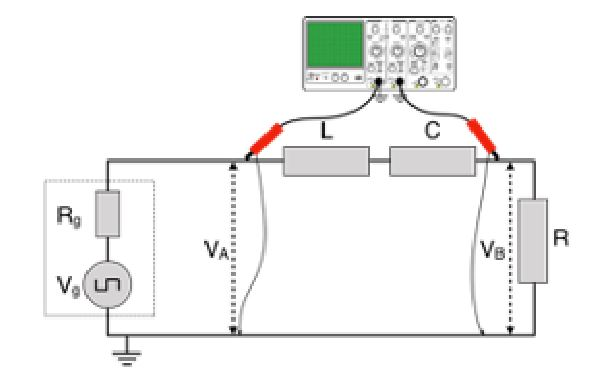
\includegraphics{configurazione_circuito_RLC.JPG}}
	\caption{Schema configurazione di circuito RLC}
	\label{fig:config_circuito_RLC}
\end{figure}

Dall'interpolazione dei grafici ottenuti nei tre casi ci aspettiamo di ricavare i valori di $\omega$ e $\gamma$ caratteristici del circuito.
\newpage

\subsection{Dati} %mancano le incertezza
Di seguito riportiamo i dati sulle componenti e la configurazione del circuito studiato:

\begin{enumerate}[itemsep=1pt]
	\item Resistenza interna oscilloscopio $R_o = (50.0\pm0.1)\Omega$
	\item Frequenza generatore $f = \SI{300}{\hertz}$
	\item Intervallo tensione $V_0= \pm (1000.0\pm0.1)\text{ mV}$

	      Di seguito riportiamo anche le formule utilizzate per la propagazione delle incertezze di $\gamma$ e $\omega$:

	      \begin{enumerate}
		      \item $ \delta_{\gamma} = \sqrt{(\frac{\partial \gamma}{\partial R} \cdot \delta R)^2 + (\frac{\partial \gamma}{\partial L}\cdot \delta L)^2} $
		      \item $ \delta_{\omega} = \sqrt{(\frac{\partial \gamma}{\partial L} \cdot \delta L)^2 + (\frac{\partial \gamma}{\partial C}\cdot \delta C)^2} $
	      \end{enumerate}
\end{enumerate}
\newpage

\subsection{Analisi dati}

\subsubsection{Regime sottosmorzato}
Per il circuito in regime sottosmorzato abbiamo utilizzato una resistenza $$R_1 =(300\pm1) \Omega $$
I dati da noi raccolti sono riportati nella tabella \ref{tab:dati_RLC_ssm} e il grafico ottenuto è riportato in figura \ref{fig:fitRLCsotto}.


\begin{figure}[h!]
	\centering
	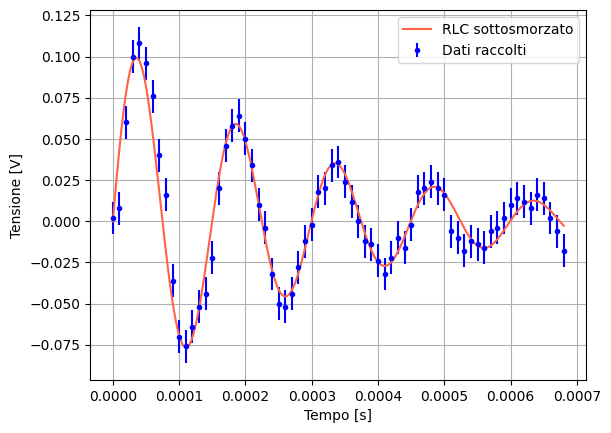
\includegraphics[width=0.8\textwidth]{RLCsotto.png}
	\caption{Grafico fit RLC sottosmorzato}
	\label{fig:fitRLCsotto}
\end{figure}

Il fit e stato eseguito con la funzione \eqref{eq: Modello sottosmorzato}.
I valori di $\gamma$ e $\omega$ calcolati con le relative incertezze sono:
\begin{align*}
    \gamma_\text{calc} & = (2.87 \pm 0.06) \cdot 10^3\ \text{Hz} \\
    \omega_\text{calc} & = (44.3 \pm 0.5) \cdot 10^3\ \text{Hz}
\end{align*}

Mentre i parametri ottenuti dal fit sono:
\begin{align*}
    \gamma_\text{attesa} & = (3.5 \pm 0.3) \cdot 10^3\ \text{Hz} \\
    \omega_\text{attesa} & = (41.9 \pm 0.2) \cdot 10^3\ \text{Hz}
\end{align*}

Eseguendo un test di compatibilità tra i valori ottenuti e quelli attesi otteniamo per $\gamma$ un $t = 2.17$ e per $\omega$ un $t = 4.49$.\\
Da questi valori, ci rendiamo conto che i valori ottenuti non sono compatibili con quelli attesi. 
Discuteremo alla fine le possibili cause di questa discrepanza. \\

\newpage

\subsubsection{Regime criticamente smorzato}
Per il circuito in regime sottosmorzato abbiamo utilizzato una resistenza $$R_2 =(3900\pm1)\ \Omega $$


\begin{figure}[h!]
	\centering
	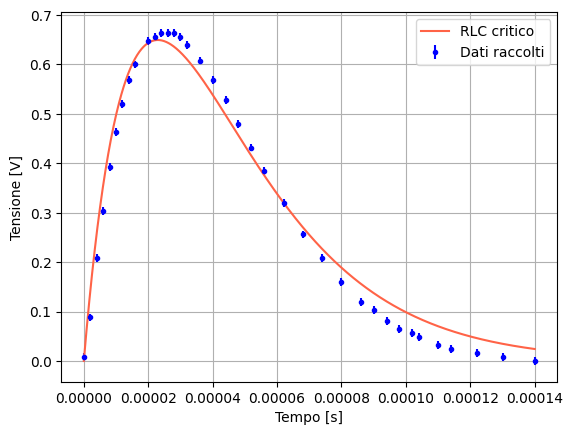
\includegraphics[width=0.8\textwidth]{RLCcritic.png}
	\caption{Grafico fit RLC critico}
	\label{fig:fitRLCcritic}
\end{figure}
\newpage

\subsubsection{Regime sovrasmorzato}
Per il circuito in regime sottosmorzato abbiamo utilizzato una resistenza $$R_3 =(10.0\pm0.1)\text{k}\Omega $$

\begin{figure}[h!]
	\centering
	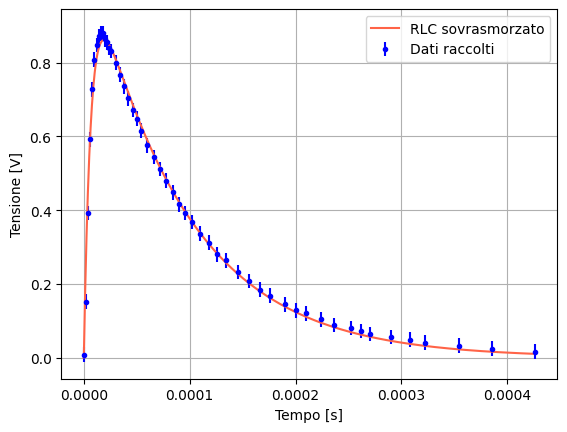
\includegraphics[width=0.8\textwidth]{RLCsovra.png}
	\caption{Grafico fit RLC sovrasmorzato}
	\label{fig:fitRLCsovra}
\end{figure}



\subsection{Conclusioni sul circuito RLC}



\section{Tabelle}

\begin{table}[htbp]
	\centering
	\caption{Dati circuito RC}
	\begin{tabular}{ccc}
		\toprule
		Tempo [ms] & Tensione - carica pos. [mV] & Tensione - carica neg. [mV] \\
		\midrule
		0.0        & 960                         & -952                        \\
		0.1        & 824                         & -824                        \\
		0.2        & 712                         & -696                        \\
		0.3        & 600                         & -600                        \\
		0.4        & 520                         & -512                        \\
		0.5        & 448                         & -440                        \\
		0.6        & 384                         & -368                        \\
		0.7        & 328                         & -320                        \\
		0.8        & 280                         & -272                        \\
		0.9        & 232                         & -224                        \\
		1.0        & 208                         & -200                        \\
		1.2        & 152                         & -144                        \\
		1.4        & 112                         & -104                        \\
		1.6        & 80                          & -72                         \\
		1.8        & 56                          & -56                         \\
		2.0        & 40                          & -40                         \\
		2.2        & 32                          & -28                         \\
		2.4        & 24                          & -16                         \\
		2.6        & 16                          & -8                          \\
		\bottomrule
	\end{tabular}
	\label{tab:dati_RC}
\end{table}

\begin{table}[htbp]
	\centering
	\caption{Dati circuito RL}
	\begin{tabular}{cc}
		\toprule
		Tempo [ms] & Tensione - carica [mV] \\
		\midrule
		0.0        & -900                   \\
		0.01       & -560                   \\
		0.02       & -360                   \\
		0.03       & -80                    \\
		0.04       & 120                    \\
		0.05       & 240                    \\
		0.06       & 340                    \\
		0.07       & 500                    \\
		0.08       & 600                    \\
		0.09       & 620                    \\
		0.1        & 680                    \\
		0.12       & 780                    \\
		0.13       & 820                    \\
		0.14       & 840                    \\
		0.15       & 860                    \\
		0.16       & 880                    \\
		0.18       & 900                    \\
		0.2        & 920                    \\
		0.22       & 940                    \\
		0.29       & 960                    \\
		\bottomrule
	\end{tabular}
	\label{tab:dati_RL}
\end{table}

\begin{table}[htbp]
	\centering
	\caption{Dati caso sottosmorzato}
	\begin{tabular}{cc}
		\toprule
		Tempo [ms] & Tensione [mV] \\
		\midrule
		0.0        & 2             \\
		0.01       & 8             \\
		0.02       & 60            \\
		0.03       & 100           \\
		0.04       & 108           \\
		0.05       & 96            \\
		0.06       & 76            \\
		0.07       & 40            \\
		0.08       & 16            \\
		0.09       & -36           \\
		0.1        & -70           \\
		0.11       & -76           \\
		0.12       & -64           \\
		0.13       & -52           \\
		0.14       & -44           \\
		0.15       & -22           \\
		...        & ...           \\
		0.66       & 2             \\
		0.67       & -6            \\
		0.68       & -18           \\
		\bottomrule
	\end{tabular}
	\label{tab:dati_RLC_ssm}
\end{table}

\begin{table}[htbp]
	\centering
	\caption{Dati caso criticamente smorzato}
	\begin{tabular}{cc}
		\toprule
		Tempo  [ms] & Tensione [mV] \\
		\midrule
		0.0         & 8.0           \\
		0.002       & 88.0          \\
		0.004       & 208.0         \\
		0.006       & 304.0         \\
		0.008       & 392.0         \\
		0.01        & 464.0         \\
		0.012       & 520.0         \\
		0.014       & 568.0         \\
		0.016       & 600.0         \\
		0.02        & 648.0         \\
		0.022       & 656.0         \\
		0.024       & 664.0         \\
		0.026       & 664.0         \\
		0.028       & 664.0         \\
		0.03        & 656.0         \\
		0.032       & 640.0         \\
		0.036       & 608.0         \\
		0.04        & 568.0         \\
		0.044       & 528.0         \\
		0.048       & 480.0         \\
		0.052       & 432.0         \\
		0.056       & 384.0         \\
		0.062       & 320.0         \\
		0.068       & 256.0         \\
		0.074       & 208.0         \\
		0.08        & 160.0         \\
		0.086       & 120.0         \\
		0.09        & 104.0         \\
		0.094       & 80.0          \\
		0.098       & 64.0          \\
		0.102       & 56.0          \\
		0.104       & 48.0          \\
		0.11        & 32.0          \\
		0.114       & 24.0          \\
		0.122       & 16.0          \\
		0.13        & 8.0           \\
		0.14        & 0.0           \\
		\bottomrule
	\end{tabular}
	\label{tab:dati_RLC_csm}
\end{table}

\begin{table}[htbp]
	\centering
	\caption{Dati caso sovrasmorzato}
	\begin{tabular}{cc}
		\toprule
		Tempo [ms] & Tensione [mV] \\
		\midrule
		0.0        & 8.0           \\
		0.002      & 152.0         \\
		0.004      & 392.0         \\
		0.006      & 592.0         \\
		0.008      & 728.0         \\
		0.01       & 808.0         \\
		0.012      & 848.0         \\
		0.014      & 872.0         \\
		0.016      & 880.0         \\
		0.018      & 880.0         \\
		0.02       & 864.0         \\
		0.022      & 856.0         \\
		0.024      & 840.0         \\
		0.026      & 832.0         \\
		0.03       & 800.0         \\
		0.034      & 768.0         \\
		...        & ...           \\
		0.354      & 32.0          \\
		0.386      & 24.0          \\
		0.426      & 16.0          \\
		\bottomrule
	\end{tabular}
	\label{tab:dati_RLC_svsm}
\end{table}


\end{document}
